\documentclass[14pt]{beamer}
\usetheme{Berkeley}
\usepackage[ngerman]{babel}
\usepackage[utf8]{inputenc}
\usepackage{graphicx}
\usepackage{pgfplots}
\usepackage{pgfplotstable}
\author{Bennet, Leonard, Jochen, Philip, Tim}
\title{Normalverteilung}
\graphicspath{{images/}}
%\setbeamercovered{transparent} 
%\setbeamertemplate{navigation symbols}{} 
\logo{
\includegraphics[scale=0.4]{logo.png}} 
%\logo{\includegraphics[scale=0.15]{logo_herder.png}} 
\institute{Herder Gymnasium Berlin} 
\date{}

\begin{document}

\begin{frame}
 \titlepage
\end{frame}

%\section{Inhalt}
%[allowframebreaks]
\begin{frame}{Inhalt}
 \tableofcontents
\end{frame}

\section{Dichtefunktionen}
\begin{frame}{Wozu eine Dichtefunktion?}
\textbf{Bisherige Berechnung}:

{\small $$ P(X \in\mathbb{A}) \, = \, \sum_{x\in A} \rho(x) $$}
\begin{itemize}

\item eignet sich nur für diskrete Wahrscheinlichkeitsverteilungen:

\begin{itemize}
\only<1>{
\item Binomial
\item Hypergeometrisch
\item Poisson
}
\only<2>{
\item[$\Rightarrow$] keine Aussage möglich für stetige Verteilungen, da $P(X \, = \, x) = 0 \, \forall X \in \mathbb{A}$
}
\end{itemize}
\end{itemize}

\end{frame}

\subsection{Definition}
\begin{frame}{Definition}
\textbf{Wahrscheinlichkeit als Flächeninhalt:}
$\varphi \colon \mathbb{R} \rightarrow [0,\infty)$ mit
$$P(X \in \mathbb{A})=\int\displaylimits_{X \in \mathbb{A}} \varphi(x)\,{\mathrm d}x$$
ist die \textbf{Wahrscheinlichkeitsdichte} der Verteilung von $X$.
\end{frame}

\subsection{Eigenschaften}
\begin{frame}{Eigenschaften}
Eigenschaften:
\begin{itemize}
\item $\forall x \in \mathbb{R}:\, \varphi(x)\geq 0$
\item $\int\displaylimits_{-\infty}^\infty \varphi\ (x)\,{\mathrm d}x = 1$
\end{itemize}
Eine Funktion $f$ ist genau dann eine Dichtefunktion, wenn diese Eigenschaften erfüllt sind.
\end{frame}

\subsection{Nutzung}
\begin{frame}{Rechnen mithilfe der Dichtefunktion}
Wahrscheinlichkeit für ein Intervall $[a,b]$:
$$P(X\in [a,b]) = \int\displaylimits_a^b \varphi\ (x)\, {\rm d}x = \Phi(b)-\Phi(a).$$
$F$ ist die sogenannte \textbf{kumulative Verteilungsfunktion} mit:
$$\Phi(x) \, = \, P(X \le x)$$
\end{frame}


\section{Standardisierung}

\begin{frame} {Standardisierung}

Standardisierung (auch Z-Transfomation) ist eine Transformation einer Zufallsvariable, z.B. X, sodass gilt: $$E(x) = \mu = 0$$ und $$V(x) = \sigma^2 = \sigma = 1$$

\end{frame}

\begin{frame} {Standardisierung}

Zunächste Erwartungswert auf Y-Achse verschieben:
$$ Z = X - \mu $$
Dann jede Verteilung auf eine Breite bringen
$$ Z = \frac{X - \mu}{\sigma} $$
Damit die Fläche gleichbleibt, gilt:
$$ Y = \sigma \cdot B_{n;p}(Z) $$

\end{frame}




\section{Approximation der Binomialverteilung}


\begin{frame}{Zusammenfassung}
$$
P(X\leq\ c) = \frac{1}{\sigma} \cdot \int\displaylimits^c_{-\infty} \varphi\ \left(\frac{t-\mu}{\sigma}\right) {\mathrm d}t
$$
mit Substitution $g(t):=\frac{t-\mu}{\sigma} \Rightarrow g'(t)=\frac{1}{\sigma}$:
$$
= \int\displaylimits^{\frac{c-\mu}{\sigma}}_{-\infty} \varphi(x) {\mathrm d}x =: \phi\ \left(\frac{c-\mu}{\sigma}\right) $$
\end{frame}

\subsection{lokaler Grenzwertsatz}
\begin{frame}{\textrm{\textsc{Gau}ß}}
Nach \textrm{\textsc{Gau}ß} ist eine dazu passende Funktion $\varphi$:
$$
\varphi(x)=b\cdot e^{-a\cdot\ x^2}
$$
Durch unsere Vereinheitlichung der Breite ist das $1\cdot \sigma$-Intervall $[-1;1]$.
\end{frame}


\begin{frame}{Was ist $a$?}
Betrachten des Graphen der Binomialverteilung zeigt uns, an $x=\pm 1$ sind Wendestellen.\\
Für $x=\pm 1$:\\
2. Ableitung: $2abe^{-a} \cdot (-1+2 a)$\\
3. Ableitung: $-4 a^{2} b e^{-a} (\pm1) (-3+2 a)$\\

Da $\varphi''(x)=0$ und $\varphi'''(x)\neq0$ muss:\\
$a=\pause\frac{1}{2}$
\end{frame}

\begin{frame}{Was ist $b$?}
Der Flächeninhalt des Graphen muss $1$ sein:
\begin{eqnarray}
1&=&\int\displaylimits^{\infty}_{-\infty} b \cdot e^{-\frac{1}{2}x^2} {\mathrm d}x \\
\Leftrightarrow \frac{1}{b}&=&\int\displaylimits^{\infty}_{-\infty} e^{-\frac{1}{2}x^2} {\mathrm d}x \\
I^2 &=& \int\displaylimits^{\infty}_{-\infty} \int\displaylimits^{\infty}_{-\infty} e^{-\frac{1}{2}x^2} e^{-\frac{1}{2}y^2} {\mathrm d}x \, {\mathrm d}y
\end{eqnarray}
\end{frame}

\begin{frame}[allowframebreaks]{Was ist $b$?}
\small
\begin{eqnarray}
I^2 &=& \int\displaylimits^{\infty}_{-\infty} \int\displaylimits^{\infty}_{-\infty} e^{-\frac{1}{2}x^2} e^{-\frac{1}{2}y^2} dx \, dy \\
&=& \int\displaylimits^{\infty}_{-\infty} \int\displaylimits^{\infty}_{-\infty} e^{-\frac{1}{2}(x^2 + y^2)} dx \, dy \\ 
&=& \int\displaylimits^{2 \pi}_{0} \int\displaylimits^{\infty}_{0} e^{-\frac{1}{2}r^2} r{\mathrm d}\varphi \, dr
\end{eqnarray}
\end{frame}

\begin{frame}[allowframebreaks]{Was ist $b$?}
\small
\begin{eqnarray}
&=& 2 \pi \int\displaylimits^{\infty}_{0} e^{-\frac{1}{2}r^2} r{\mathrm d}r \\
&=& 2 \pi \begin{bmatrix}-e^{-\frac{1}{2} r^2} \end{bmatrix}^\infty_0 = 2 \pi\\
\Rightarrow b&:=&\frac{1}{\sqrt{2\pi}}
\end{eqnarray}
\end{frame}


\begin{frame}{\textrm{\textsc{Gau}ß}sche Normalverteilung}
Damit können wir dann sagen:
$$
1= \lim\limits_{x \to \infty} (\Phi(x)) =  \int\displaylimits^{\infty}_{-\infty} \varphi(x) {\mathrm d}x = \int\displaylimits^{\infty}_{-\infty} \frac{1}{\sqrt{2\cdot \pi}} \cdot e^{-\frac{1}{2}x^2} {\mathrm d}x
$$
$\varphi(x)$: \textrm{\textsc{Gau}ß}sche \textbf{Dichtefunktion}\\
$\Phi(x)$:  \textrm{\textsc{Gau}ß}sche \textbf{Summenfunktion}
\end{frame}

\section{Die Integralfunktion}
\begin{frame} {Die Integralfunktion}

Die Integralfunktion soll liefern:
$$ \lim_{n \rightarrow \infty} P\left(\frac{X_n-n\cdot\ p}{\sqrt{n\cdot\ p\cdot(1-p)}} \le X\right) = \phi(x) $$

Allgemein geschrieben:
$$ \lim_{n \rightarrow \infty} P\left(\frac{X_n-\mu}{\sigma} \le X\right) = \phi(x) $$

\end{frame}

\begin{frame} {Die Integralfunktion}

Wie kann man das ausrechnen?

\end{frame}

\begin{frame} {Die Integralfunktion}

$$ \phi(x) = \int_{-\infty}^x \varphi(t)dt $$

\end{frame}

\begin{frame} {Die Integralfunktion}

Beweis:

 \begin{itemize}
  \item Aufsummieren von unendlich kleinen Spalten (da $n \rightarrow   \infty$)
  \item Genau dieser Grenzwert ist das Integral
  \item Daraus folgt: $ P(X \in ] \mu - n \cdot \sigma, \mu + n \cdot \sigma[) = \int_{-n}^{n}\varphi(t)dt $
 \end{itemize}

\end{frame}

\begin{frame} {Die Integralfunktion}

Beweis:

 \begin{itemize}
  \item Dann geht die untere Schranke nach $ - \infty $
  \item Die Formel ist dann: $ P(X \in ] -\infty, \mu + n \cdot \sigma[) = \int_{-\infty}^n\varphi(t)dt $
  \item Zudem ist $ X \in ]-\infty, \mu + n \cdot \sigma[ \Leftrightarrow X < \mu + n \cdot \sigma $
 \end{itemize}

\end{frame}

\begin{frame} {Die Integralfunktion}

 $$ X < \mu + n \cdot \sigma \Leftrightarrow $$ $$ X - \mu < n \cdot \sigma \Leftrightarrow $$ $$ \frac{X - \mu}{\sigma} < n \Leftrightarrow $$
 In der Funktion ist wird $ n \rightarrow x $ und $ X \rightarrow X_n $
 Das Ergebnis ist:
 $$ P\left(\frac{X_n - \mu}{\sigma}\right) = \int_{-\infty}^n\varphi(t)dt  $$

\end{frame}

\section{Anwendung der Integralfunktion}
\begin{frame} {Anwendung der Integralfunktion}

Beispiel:
\begin{itemize}
 \item p = 0,035
 \item n = 1100
\end{itemize}

\end{frame}

\begin{frame} {Anwendung der Integralfunktion}

Beispiel:
\begin{itemize}
 \item p = 0,035
 \item n = 1100
 \item $\mu = 0,035 \cdot 1100 = 38,5 $
\end{itemize}

\end{frame}

\begin{frame} {Anwendung der Integralfunktion}

Beispiel:
\begin{itemize}
 \item p = 0,15
 \item n = 1100
 \item $\mu = 0,15 \cdot 1100 = 165 $
 \item $\sigma$ = $\sqrt{1100 \cdot 0,15 \cdot 0,85}$ = $\sqrt{140,25} \approx 11,84$ 
\end{itemize}
 Achtung: $\sigma \ge 3$ bzw. $\sigma^2 = V \ge 9$!

\end{frame}

\begin{frame} {Anwendung der Integralfunktion}

Beispiel:
\begin{itemize}
 \item a) $P(X \le 180)$
 \item b) $P(X < 121)$
 \item c) $P(170 < X)$
 \item d) $P(150 < X_n \le 180)$
\end{itemize}

\end{frame}

\begin{frame} {Anwendung der Integralfunktion}

Beispiel a):
 
 $$P(X\le180)$$
 $$P(X_n \le 180) =  \phi\left(\frac{X_n - \mu}{\sigma}\right)$$
 $$ \phi(\frac{180 - 165}{11,84}) = \phi(1,27) $$

\end{frame}

\begin{frame} {Anwendung der Integralfunktion}
 
 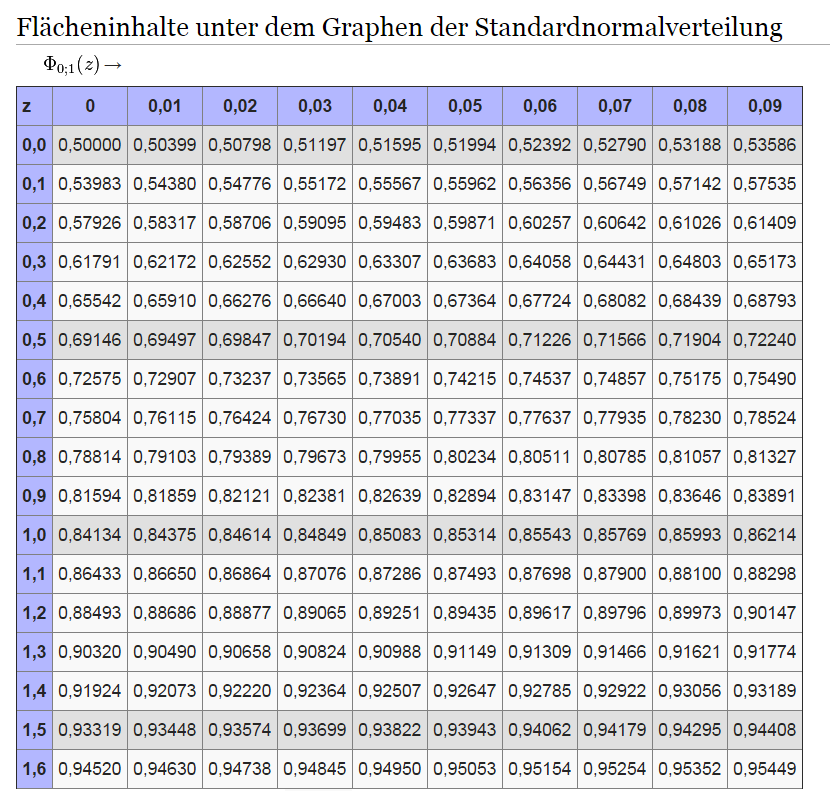
\includegraphics[width=7.0cm]{TabelleNormalverteilung.png}

\end{frame}
\begin{frame} {Anwendung der Integralfunktion}

Beispiel b):
 
 $$P(X_n < 121) \rightarrow P(X_n \le 120)$$
 $$P(X_n \le 120) =  \phi\left(\frac{X_n - \mu}{\sigma}\right)$$
 $$ \phi\left(\frac{120 - 165}{11,84}\right) = \phi(-3,8) $$
 
 Was nun?

\end{frame}
\begin{frame} {Anwendung der Integralfunktion}
 
 Es gilt:
 $$ \phi(x) = 1 - \phi(-x) $$

\end{frame}

\begin{frame} {Anwendung der Integralfunktion}
 
 $$P(X_n < 121) \rightarrow P(X_n \le 120)$$
 $$P(X_n \le 120) =  \phi\left(\frac{X_n - \mu}{\sigma}\right)$$
 $$ \phi\left(\frac{120 - 165}{11,84}\right) = \phi(-3,8) $$
 $$ \phi(-3,8) = 1 - \phi(3,8)$$

\end{frame}

\begin{frame} {Anwendung der Integralfunktion}

 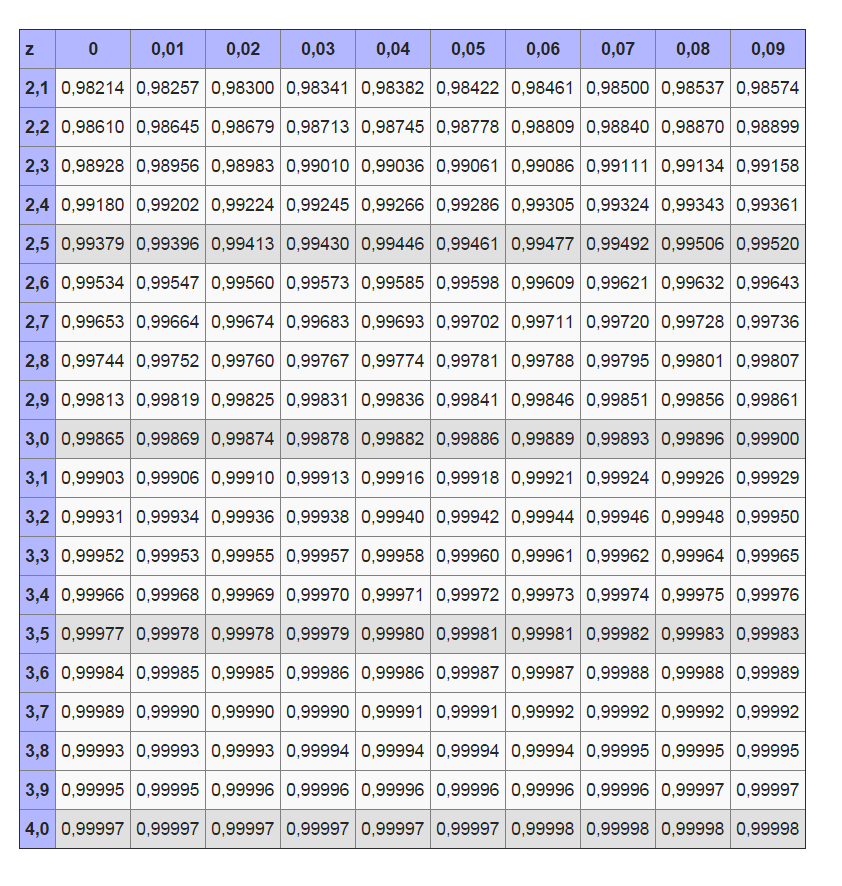
\includegraphics[width=7.0cm]{TabelleNormalverteilung2.png}

\end{frame}

\begin{frame} {Anwendung der Integralfunktion}

Beispiel c):
 
 $$P(170 < X_n)$$
 $1 - P(X_n \le 170)$
 Somit: $$P(X_n \le 170) =  \phi\left(\frac{X_n - \mu}{\sigma}\right)$$
 $$ \phi\left(\frac{170 - 165}{11,84}\right) = \phi(0,42) $$

\end{frame}

\begin{frame} {Anwendung der Integralfunktion}
 
 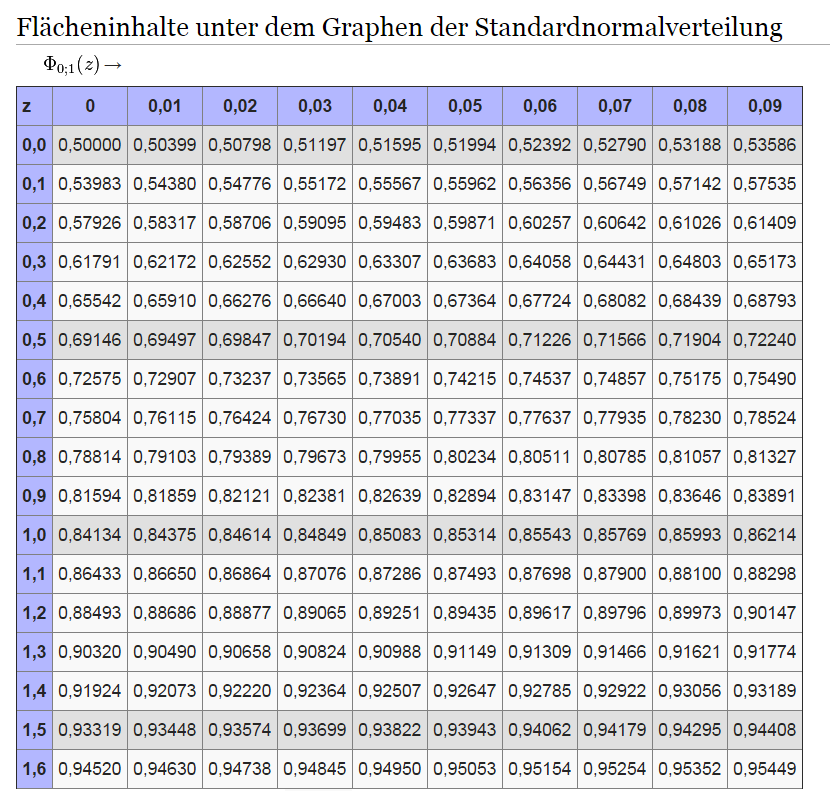
\includegraphics[width=7.0cm]{TabelleNormalverteilung.png}

\end{frame}

\begin{frame} {Anwendung der Integralfunktion}

Beispiel d):
 
 $$P(150 < X_n \le 180)$$
 $$P(X_n \le 180) - P(X_n \le 180)$$

\end{frame}

\begin{frame} {Anwendung der Integralfunktion}
 
 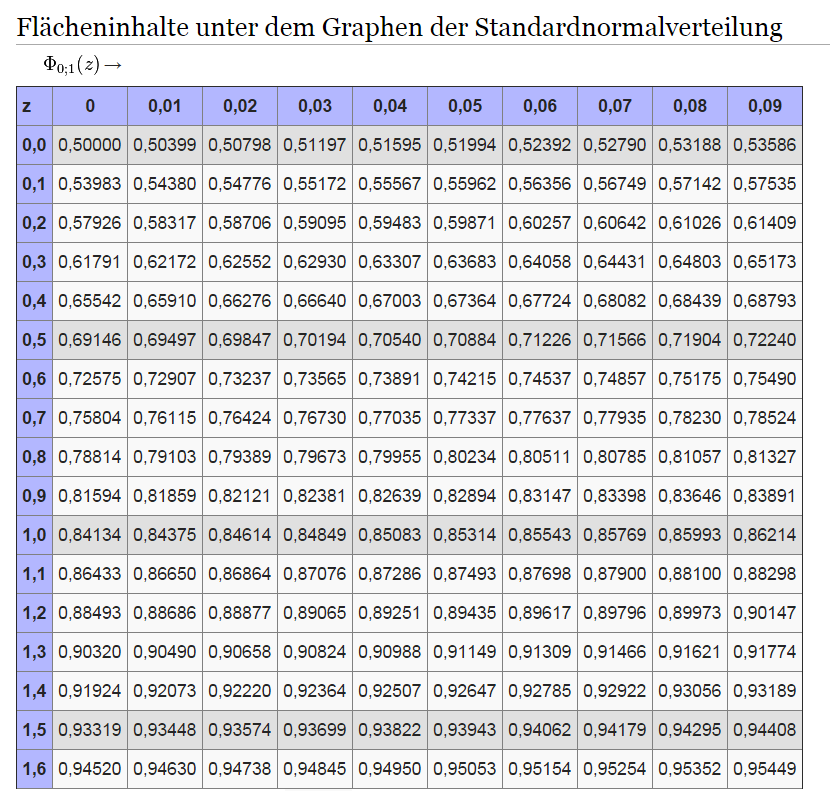
\includegraphics[width=7.0cm]{TabelleNormalverteilung.png}

\end{frame}

\section{k-$\sigma$-Intervalle}

\begin{frame}{k-$\sigma$-Intervalle}

Die Wahrscheinlichkeit ($P$), dass Ereignisse in einer $k$-$\sigma$-Umgebung liegen:
$ P(|X-p|\le k\cdot\sigma) = P(\mu-k\cdot\sigma\le X \le \mu + k\cdot\sigma)$\\
$ = P\left(\frac{\mu-k\cdot\sigma - \mu}{\sigma}\le \frac{X - \mu}{\sigma}\le \frac{\mu + k\cdot\sigma - \mu}{\sigma}\right)$\\
$ = P(-k \le Z \le k)$\\
$ \approx \phi(k) - \phi(-k)$\\
$ = \phi(k) - (1 - \phi(k))$\\
$ = \phi(k) + \phi(k) - 1$\\
$ = 2\phi(k)- 1$\\

\end{frame}

\begin{frame}{k-$\sigma$-Intervalle}

Das kann für $ k = {0;1;2;...}$ entsprechend eingesetzt werden.
 \\
Ergebnisse (Auswahl):
 \\
$ P(|X-p|\le \sigma) \approx 68,27$ \%\\
$ P(|X-p|\le 2\cdot\sigma) \approx 95,45$ \%\\
$ P(|X-p|\le 3\cdot\sigma) \approx 97,73$ \%

Vgl. Tschebyschow:

$ P(|X-p|\le 2\cdot\sigma) \approx 75$ \%\\
$ P(|X-p|\le 3\cdot\sigma) \approx 88$ \%\\

\end{frame}

\section{Ausblick: Zentraler Grenzwertsatz}

%\begin{frame}

%Seien $X_1, X_2, X_3, ...$ eine Folge von Zufallsvariablen, die auf dem selben Wahrscheinlichkeitsraum alle dieselbe Verteilung aufweisen und unabhängig sind. Weiter seien $\mu$ und $\sigma > 0$ existent.

%Dann betrachten wir eine standardisierte Zufallsvariable:
%$$ Z_n = \sum_{i = 0}^n(X_i)$$

%\end{frame}

\begin{frame}{Zentraler Grenzwertsatz}
$X_1, X_2, X_3, ...$ eine Folge von Zufallsvariablen mit
\begin{itemize}
\item selbe Verteilung bei gleichem Wahrscheinlichkeitsraum
\item unabhängig
\item es existieren $\mu$ und $\sigma >0$
\end{itemize}
Wir betrachten eine standardisierte Zufallsvariable:
$$ Z_n = \sum_{i = 1}^n(X_i)$$
\end{frame}

\begin{frame}{Zentraler Grenzwertsatz}
%Dann besagt der Zentrale Grenzwertsatz, dass die Verteilungsfunktion von $Z_n$ für $n \rightarrow \infty$ punktweise gegen die Verteilungsfunktion der Normalverteilung $\phi_{\mu;\sigma}(X)$ konvergiert. 
Dann:\\
Die Verteilungsfunktion von $Z_n$ konvergiert für $n \to \infty$ punktweise gegen die Verteilungsfunktion der Normalverteilung
$$\phi_{\mu;\sigma}(X)$$

\end{frame}

%\section*{Vielen Dank!}
\section*{Vielen Dank}
\begin{frame}{Vielen Dank!}
\begin{center}
\parskip 15pt
Vielen Dank für's Zuhören!
\end{center}
\end{frame}

\end{document}
